\documentclass[a4paper,12pt]{article}
    \usepackage[utf8]{inputenc}
    \usepackage[T1]{fontenc}
    \usepackage[english]{babel}
    \usepackage{graphicx}
    \usepackage{geometry}
    \geometry{a4paper,
                 tmargin = 35mm, 
                 lmargin = 25mm,
                 rmargin = 30mm,
                 bmargin = 30mm}
    \usepackage{mathtools}
    \usepackage{amsmath} % or simply amstext
	\newcommand{\angstrom}{\textup{\AA}}
    \usepackage{color}
    \usepackage{setspace}
    \usepackage{enumitem}
    \usepackage{amsmath,amssymb}
    \usepackage{float}
    \usepackage{listings}
    
    \usepackage{indentfirst}
	\usepackage{subfig}
	    
    \renewcommand\thesection{\Roman{section}.}
    \renewcommand\thesubsection{\thesection\arabic{subsection}}
    \renewcommand\thesubsubsection{}
    
\begin{document}

\linespread{1.2}

\begin{titlepage}

	\centering
	{\scshape\LARGE ELTE Faculty of Science\par}
	\vspace{2cm}
	
\includegraphics[width=0.66\textwidth]{./dslogo.png}
	\par\vspace{4cm}
	{\scshape\Large Photometric redshift estimation\par}
	\vspace{.5cm}
	{\large\itshape Alex Olar \par}
	\vfill
	{\large 2018 \par}

\end{titlepage}

\onehalfspacing

\begin{abstract}
	\par After reading several papers on the topic I had to reevaluate
	the methods that were used and test their accuracy and reimplement
	the majority of them.
	\par Photometric redshift estimation is a highly popular area and is
	still very important today as a huge portion of the sky is not accurately
	measured or measured at all by spectroscopists so finding the redshift of
	available data and developing a good method and tool to accurately predict
	it would be highly beneficial for all.
	\par My task is to get familiar with these concepts and try to find the
	best among them with machine learning techniques and general clustering
	algorithms.
\end{abstract}

\tableofcontents

\newpage

\section{The problem}

\par The Sloan Digital Sky Survey has done an imaging
survey in five optical bands which was later on followed
by a spectroscopic measurement where more than a million galaxy
was observed. The optical bands were matched with the right spectroscopic
data and magnitudes and redshifts were calculated. It is all stored
in a huge database which is available on the SDSS SkyServer \cite{server}.

\par The magnitudes and petrosian magnitudes, which is corrected for
each galaxy type and by other factors as well, can be found in this database
with the appropriate errors and the spectroscopic data can be joined to it as
well.

\par The database is a simple SQL database and scripts can be submitted
to the CasJobs page on SkyServer to run and get the data from the servers.
Therefore anyone has access to it freely and is able to do his/her
experiments on it. I acquired most of my data by running this script:

\lstset{language=SQL}
\lstset{frame=lines}
\lstset{caption={SQL script on CasJobs}}
\lstset{basicstyle=\footnotesize}
\begin{lstlisting}
    SELECT
  p.modelMag_u as m_u,
  ...
  p.modelMag_z as m_z,
  p.petroMag_u as pm_u,
  ...
  p.petroMag_z as pm_z,
  p.modelMag_u-p.extinction_u-p.modelMag_g+p.extinction_g as ug,
  ...
  p.modelMag_i-p.extinction_i-p.modelMag_z+p.extinction_z as iz,
  p.petroMag_u-p.extinction_u-p.petroMag_g+p.extinction_g as p_ug,
  ...
  p.petroMag_i-p.extinction_i-p.petroMag_z+p.extinction_z as p_iz,
  s.z as z into mydb.MyTable from PhotoObj AS p
  JOIN SpecObj AS s ON s.bestobjid = p.objid
WHERE
  p.probPSF=0 AND
  p.petroMagErr_u/p.petroMag_u BETWEEN 0 AND 0.05 AND
  ...
  p.modelMagErr_z/p.modelMag_z BETWEEN 0 AND 0.05
\end{lstlisting}

\par The \textbf{WHERE} clause states that I selected only
galaxies from the SDDS DR7 database and all the acquired data
have less then 5\% error. This procedure resulted in 750'000
lines, although to run my simulations I only used a tiny bit of
this in order to be able to make it run faster and handle errors
in run time.

\par On this data set, I had to do the photometric
redshift estimation. In order to do this I had to try
different clustering algorithms myself and after that I
had to move on with implementing the procedure from Róbert
Beck's article \cite{beck}. I got familiar with the problem
by scanning through professor Csabai's article \cite{csabai}
and implementing some of the algorithms that could be found
there and plotting the galaxy distributions by color indices.

\section{Empirical methods}

\subsection{Approach}

\par The acquired data was in \textit{.csv} file format
which can be easily read and processed by \textit{pandas}
package \cite{pandas} in \textmd{Python}. After reading the data
I made the plots for model and petrosian magnitudes as well. The
following figures will show the differences in color space:

\begin{figure}[H]
	\centering
	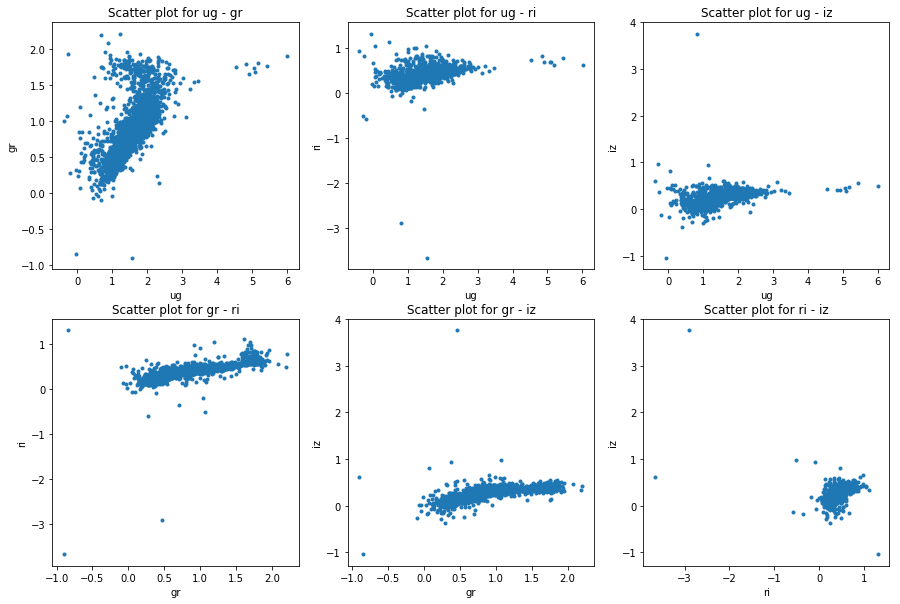
\includegraphics[width=1.\textwidth]{./modelmagscolor.png}
	\caption{ Model magnitudes for color space diagrams }
\end{figure}

\begin{figure}[H]
	\centering
	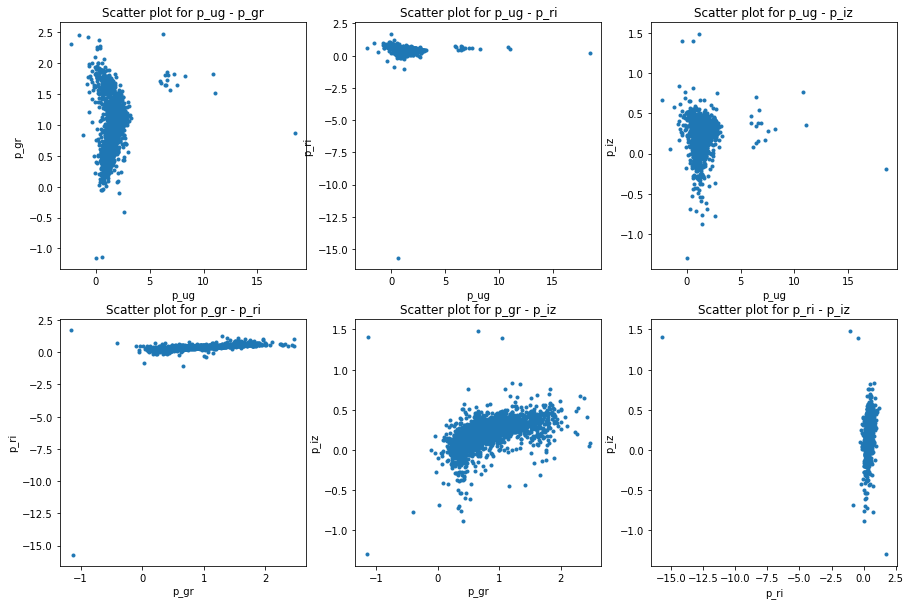
\includegraphics[width=1.\textwidth]{./petromagscolor.png}
	\caption{ Petrosian magnitudes for color space diagrams corrected for extinction }
\end{figure}

\par I consider this data as comparison baseline for the template
data I have later on generated. Not only does the data need to cover
the whole color space but also it should not contain too many outlier
galaxies. This is taken care of as I only selected data points with
small errors. A train-test split was done in 80\%-20\%.

\subsection{Implementations, results}

\par First of all I used a naive k-Nearest neighbor method. A brief introduction
to the algorithm is the following: there's a huge labeled dataset, the training
dataset, with the appropriate color bands and redshift values. Using the test dataset
we are looking for its k nearest neighbors and setting its redshift value
to the mean of the nearest neighbors.

\par On the other hand, I mostly used the algorithms from the \textit{sklearn} package
\cite{sklearn} which includes KNN, support vector machine (SVM) and random forest algorithms, which
are very well optimized and are using great tricks to store and handle data efficiently.
For example, the KNN algorithm provided by \textit{sklearn} used \textit{kd-trees}, a data
structure that is fast to search and build from training data, therefore it is fast do find
the nearest neighbors of any given point after training the model.

\par For validation purposes the training and test sets are gathered from the
same source and both have measured redshift values. Therefore I was able to generally
say something about the goodness of my predictive models, by predicting the acquired and
measured redshift values. Cross validation

\par Results are shown on the plots and values below:

\begin{figure}[H]
	\centering
	\begin{minipage}{0.5\textwidth}
		\centering
		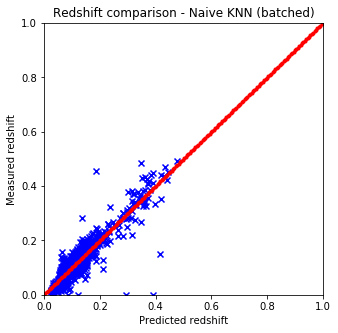
\includegraphics[width=0.95\textwidth]{./algos1.png}
		\caption{ Naive KNN - slow, accurate }
	\end{minipage}\hfill
	\begin{minipage}{0.5\textwidth}
		\centering
		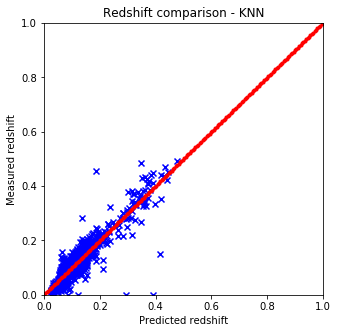
\includegraphics[width=0.95\textwidth]{./algos2.png}
		\caption{ sklearn KNN - fast, accurate }
	\end{minipage}
\end{figure}

\begin{figure}[H]
	\centering
	\begin{minipage}{0.5\textwidth}
		\centering
		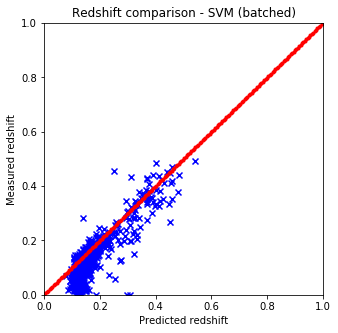
\includegraphics[width=0.95\textwidth]{./algos3.png}
		\caption{ SVM - slow, not accurate }
	\end{minipage}\hfill
	\begin{minipage}{0.5\textwidth}
		\centering
		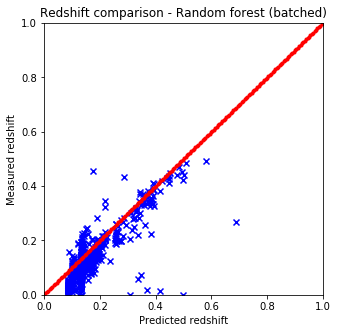
\includegraphics[width=0.95\textwidth]{./algos4.png}
		\caption{ Random forest - slow, not accurate }
	\end{minipage}
\end{figure}

\par It is quite easy to see that the KNN algorithm is the best for the problem since the predicted
redshift values for the training set fit well the measured redshift values of the training set.
However, my naive KNN is way slower than the one provided by \textit{sklearn} and needs to be batched
for a huge input data file, thus gets worse and does not scale well. The support vector machine and
the random forest algorithms does not predict redshifts very well for values lower than 0.15, thus
later on I am going to use \textit{sklearn}'s KNN.

\par Below a comparison can be seen for a five split cross validation for \textbf{k = 7} nearest
neighbors. For this purpose a ten thousand line 5\% error limited data file was used.


\begin{table}[H]
	\centering
	\begin{tabular}{|c|c|c|c|}  \hline
		\textbf{Method}        & \textbf{MAE}                   & \textbf{MSE}                   & \textbf{Duration [s]} \\ \hline
		Random forest          & 0.04296 $\pm$ 0.00362          & 0.00850 $\pm$ 0.00388          & 31.01                 \\ \hline
		Support vector machine & 0.05080 $\pm$ 0.00328          & 0.00809 $\pm$ 0.00322          & 1.07                  \\ \hline
		\textbf{KNN}           & \textit{0.02364 $\pm$ 0.00127} & \textit{0.00596 $\pm$ 0.00348} & \textbf{2.28}         \\ \hline
		Naive KNN              & 0.02364 $\pm$ 0.00127          & 0.00596 $\pm$  0.00348         & \textit{612.25}       \\ \hline
	\end{tabular}
	\caption{Comparison of different algorithms on the example dataset}
\end{table}

\par The best and worst values are presented in italics. It can be clearly seen that the best
option is the KNN algorithm, using kd-trees from \textit{sklearn}. It can be seen that without
batching the naive KNN gives the same results but is much slower.

\section{ Local linear regression}

\subsection{Theory}

\par According to the article of Beck \cite{beck} I was able to implement a local
linear regression method by finding the k nearest neighbor of a test data point and
fitting a linear function on those with the least-squares method. The process is the
following: at first I needed to acquire the N(=100/166) nearest neighbors, secondly
a least squares fitting must have been done, thirdly a prediction for the fitted nearest
neighbors must be done to exclude the outlying values, finally the redshift must be
predicted with the outlying values left out.

\par I am applying normalization on the data points as well, therefore, I am subtracting
the mean of the data points and dividing by the standard deviation. This ensures that
my data is correctly fitted and is less prone to rounding errors. The applied
equations are the following:

\begin{align}
	z_{pred, i} = c_{i} + \vec{a}_{i}\vec{d}_{i} \\
	\chi_{i}^{2} = \sum_{j \in NN} \frac{(z_{measured, j} - c_{i} - \underbar{a}_{i}\underbar{d}_{j})^{2}}{w_{j}}
\end{align}

\par Where, according to Beck $\underbar{d}_{i}$ contains the $r$ band and all the color
indices $ug$, $gr$, $ri$, $iz$. The photometric redshift is predicted by doing a linear
fit with the \textit{sklearn} package by minimizing the $\chi^{2}$ for each index.

\par After the fit the k nearest neighbors are gathered and they must be predicted with
the local linear model. If their relative error calculated below is three times bigger, than
the deviation of the predicted value, from the measured value, the fitted data point is
dropped and the fit must be done again without the outlying neighbors. The weights ($w_{j}$)
are all considered to be ones, however a weighted nearest neighbor algorithm can be fitted as
well by using the standard $w_{j} = \frac{1}{dist(point, data_{j})}$ weight metrics.
\begin{align}
	\delta z_{phot, i} \approx \sqrt{\sum_{j \in NN} \frac{(z_{measured, j} - c_{i} - \underbar{a}_{i}\underbar{d}_{j})^{2}}{k}} \\
	3\delta z_{phot, i} < |z_{meausered, j} - c_{i} - \underbar{a}_{i}\underbar{d}_{j}|
\end{align}

\subsection{Results}

\par By implementing this algorithm I acquired the following results:

\begin{figure}[H]
	\centering
	\begin{minipage}{0.5\textwidth}
		\centering
		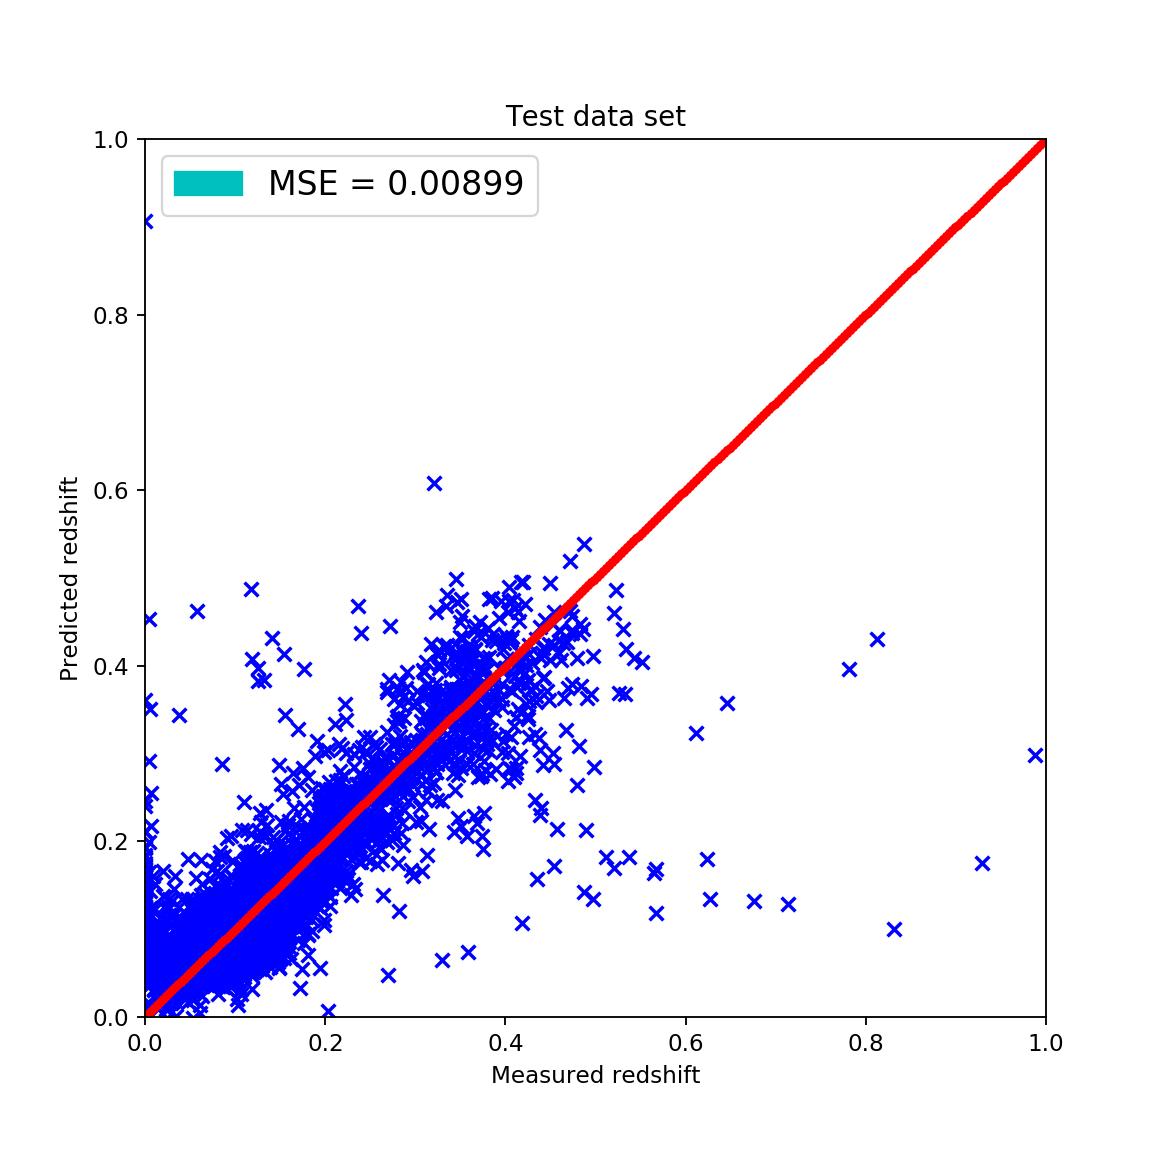
\includegraphics[width=0.95\textwidth]{./beck-default.png}
		\caption{ Result with k = 166 }
	\end{minipage}\hfill
	\begin{minipage}{0.5\textwidth}
		\centering
		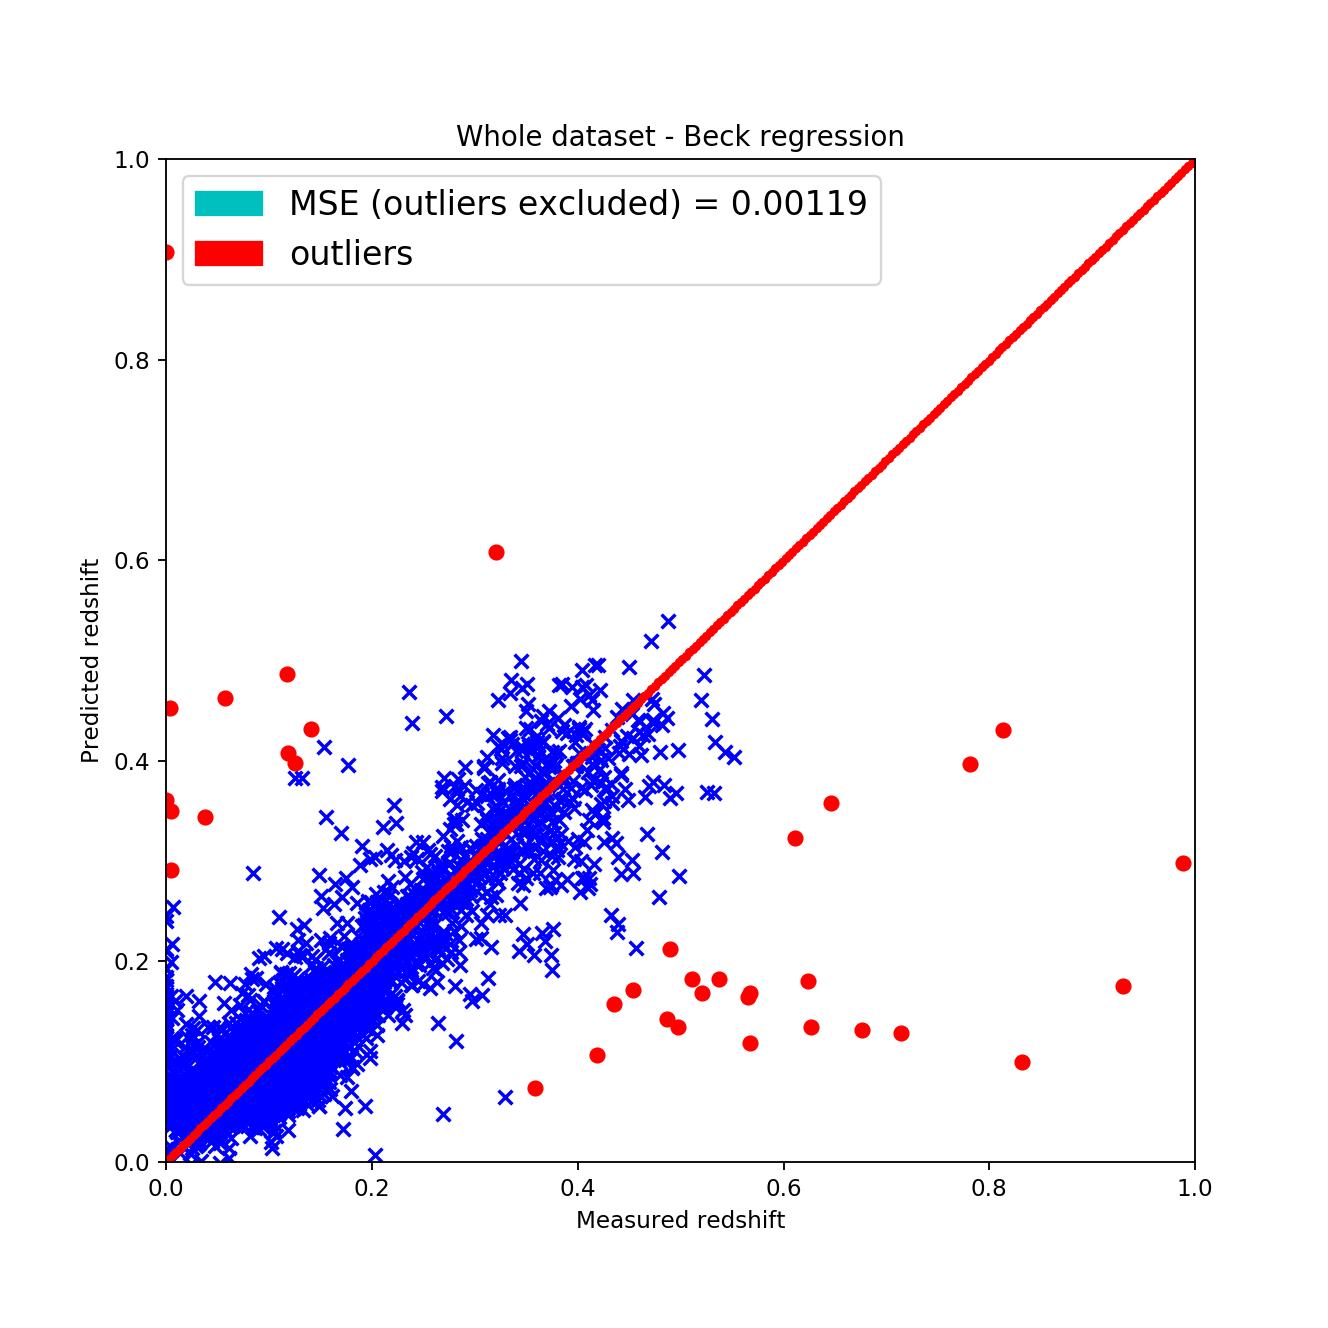
\includegraphics[width=0.95\textwidth]{./beck-outliers.png}
		\caption{ Outliers excluded k = 166 }
	\end{minipage}
\end{figure}

\par The train-test splits were made using a 20\%-80\% split by randomly
shuffling the dataset for acquiring the most appropriate results. However,
the fitted data can be qualitatively described by the these statements:

\begin{itemize}
	\item the wave-like shape has disappeared around the 45$^{\circ}$,
	      $z_{pred} = z_{measured}$ line this is considered good since it shows
	      that the fit is actually showing signs of linearity
	\item the mean squared error is approximately the same as with the KNN
	      algorithm but after excluding the outliers it gets way better
	\item analyzing the results of the cross validation it cannot be said that this
	      approach is the best among all other since it isn't the most stable regarding
	      the standard deviations of MAE and MSE
\end{itemize}

\begin{table}[H]
	\centering
	\begin{tabular}{|c|c|c|c|}  \hline
		\textbf{Method} & \textbf{MAE}          & \textbf{MSE}          & \textbf{Duration [s]} \\ \hline
		KNN             & 0.02438 $\pm$ 0.00035 & 0.00517 $\pm$ 0.00011 & \textbf{12.12}        \\ \hline
		Beck's method   & 0.0267 $\pm$ 0.00042  & 0.0069 $\pm$ 0.00071  & 178.6                 \\ \hline
	\end{tabular}
	\caption{Comparison of sklearn's KNN and Beck's local linear regression}
\end{table}

\par The downside of the local linear regression fit is that is much slower than KNN,
although that is not really considered bad since we have better computers and generally
we don't need fast algorithms, we need algorithms that finish in reasonable time and give
the best results. It is very hard to say that the standard KNN algorithm is better
since the scientific method gave a more linear result not by MAE or MSE but by pure
reasoning according to the plots. (The cross validation was re-done for the KNN algorithm
using the same 20\%-80\% split, shuffling and method.)

\section{ Template fitting}

\par After completing the tasks above I headed to experiment with the so called
template fitting where theoretical galaxy spectra is generated with different
redshift values and best fits are selected compared to real, measured data points.
This way it is possible to generate a model without having too many measured values.
However, this method is considered much worse than the others above, and according to
my calculations it is indeed much worse.

\par Photometric redshift is defined as:

\begin{align}
	z = \frac{\lambda_{observed} - \lambda_{emitted}}{\lambda_{emitted}} \\
	\lambda_{observed} = \lambda_{emitted}(1+z)
\end{align}

\par Where the emitted spectrum is given from a template set. For this reason
I used \textbf{299} spectrum files with wavelength and spectral value pairs. After applying
the filters AB magnitudes had been calculated.

\begin{equation}
	F = \frac{\int S(\lambda)r(\lambda)\lambda d\lambda}{c\int r(\lambda)\frac{1}{\lambda}d\lambda}
\end{equation}

\par Whereas c is the speed of light $S(\lambda)$ is the spectral function and $r(\lambda)$
is the filter function which was acquired from voservices \cite{voservices}. Some of
the selected spectral functions and all the filters are presented below:

\begin{figure}[H]
	\centering
	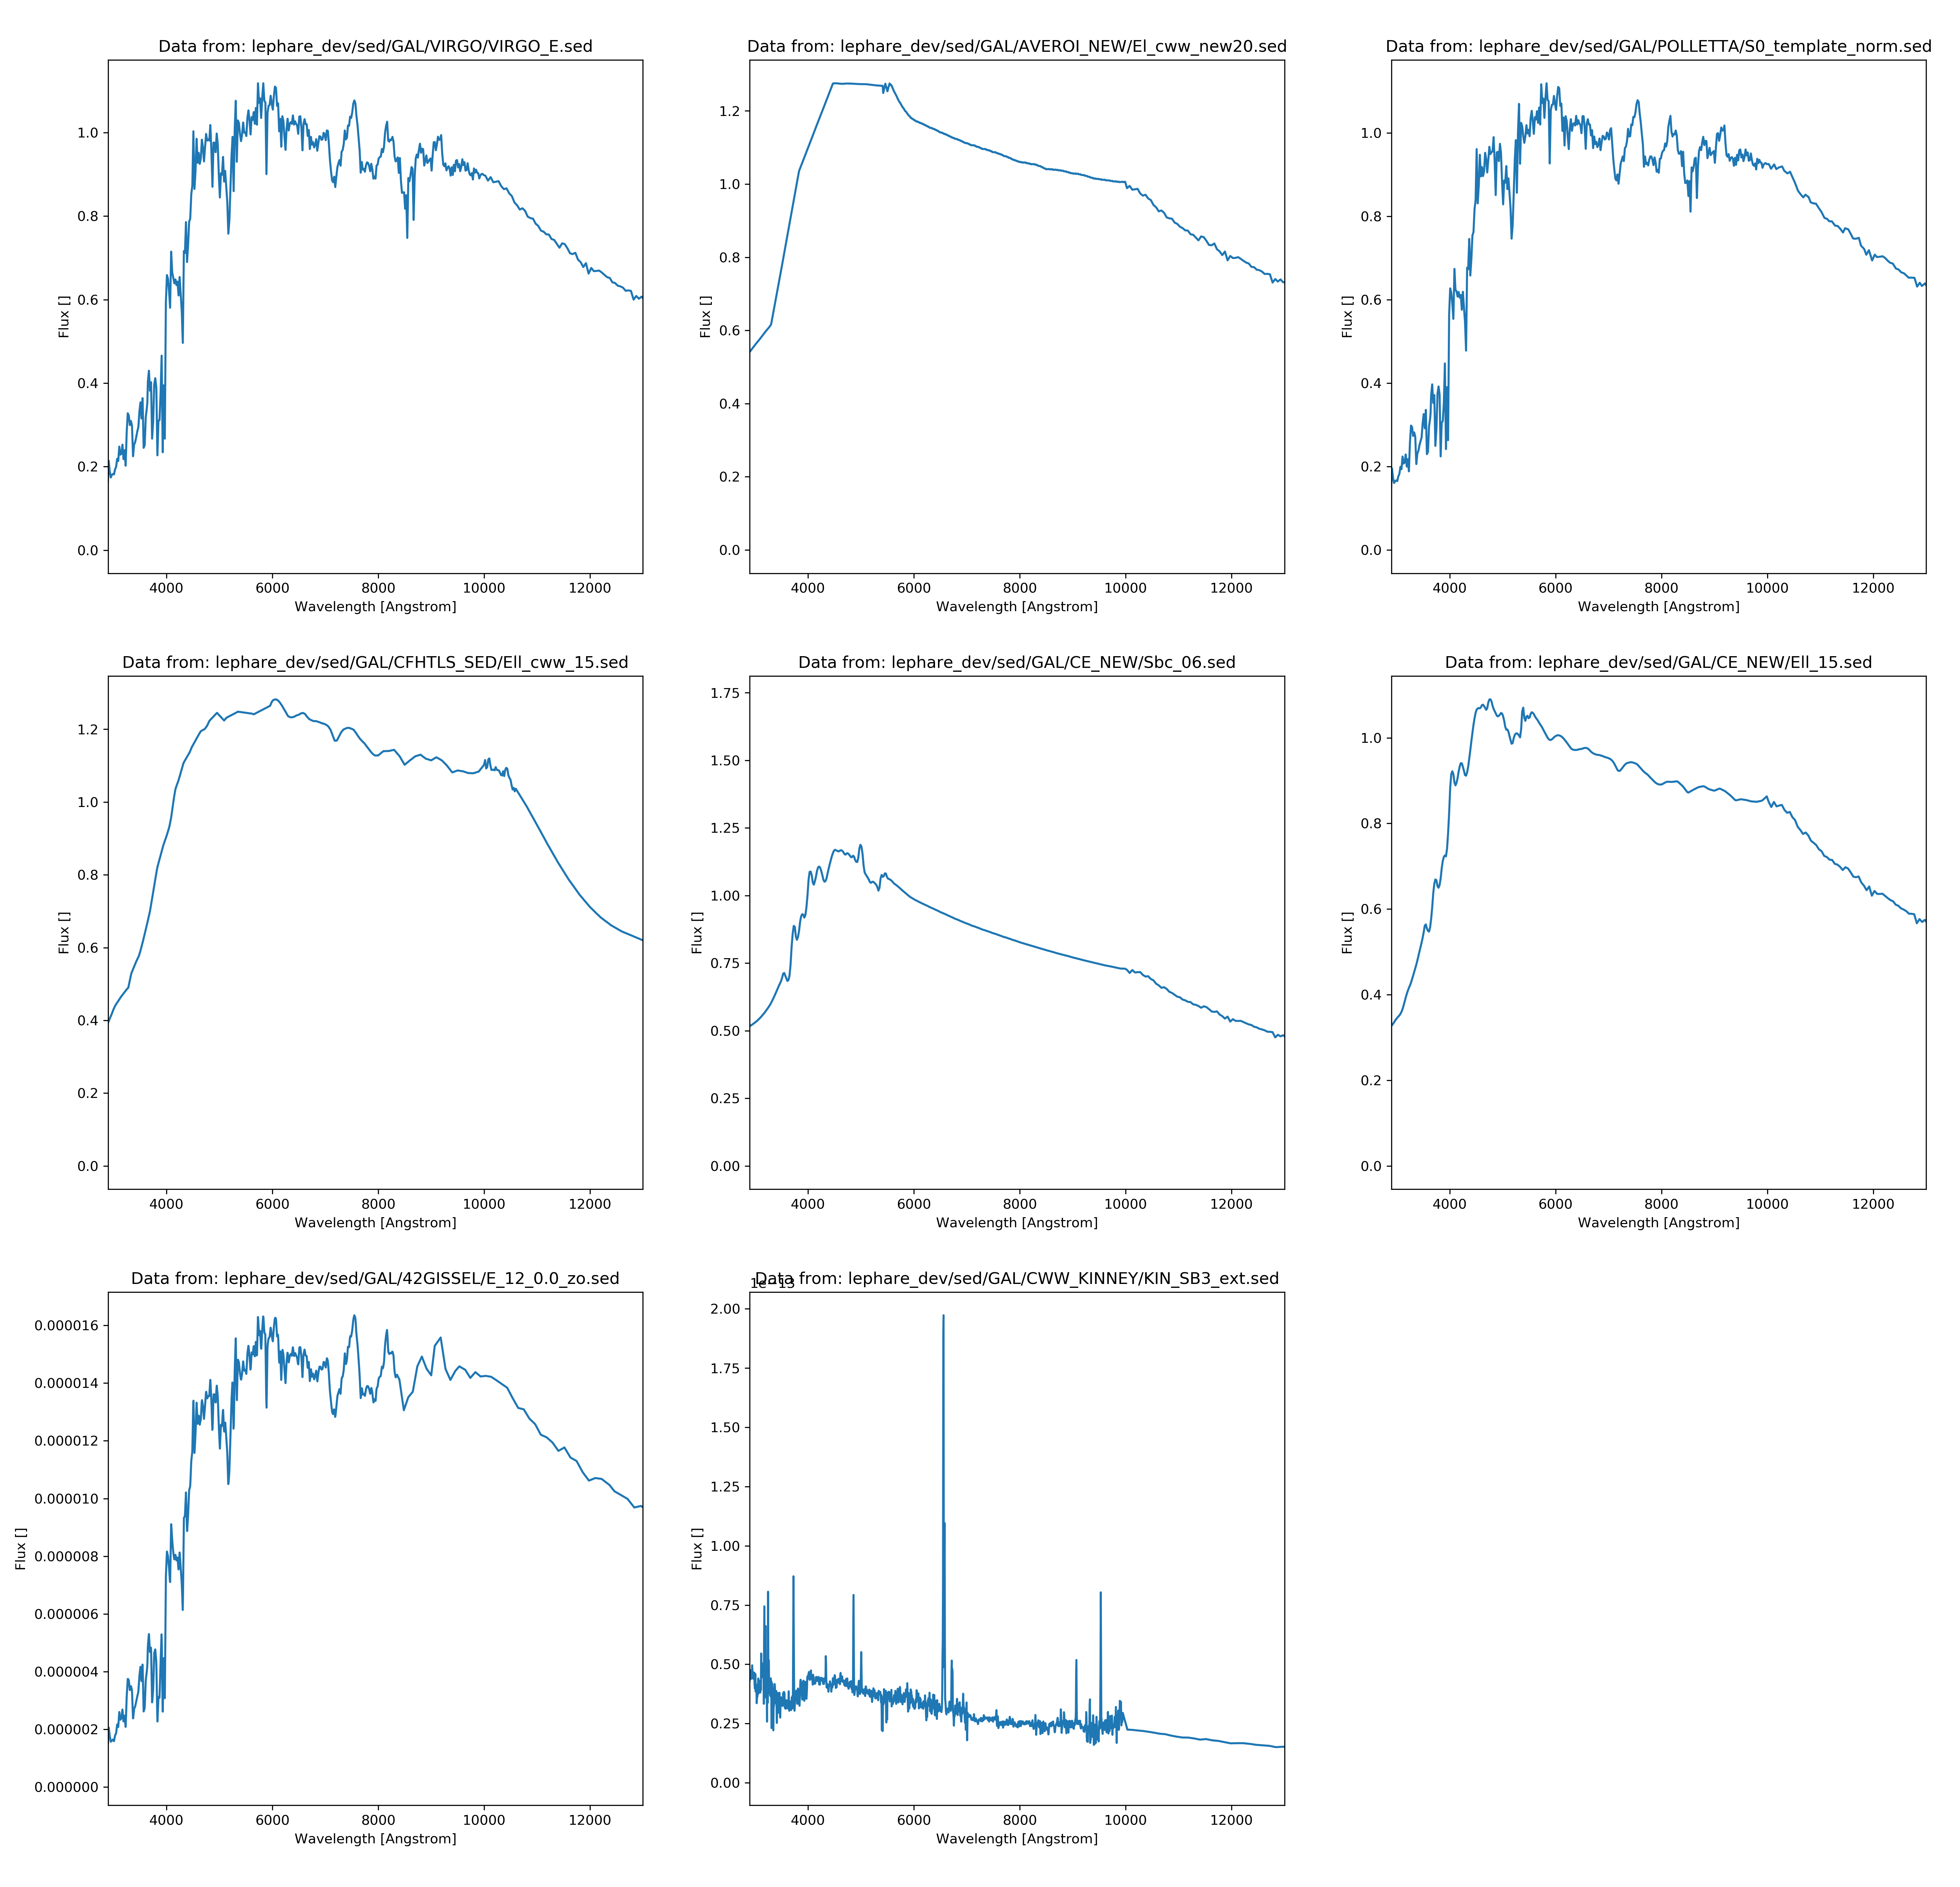
\includegraphics[width=0.66\textwidth]{./example-spectra.png}
	\caption{ Model magnitudes for color space diagrams }
\end{figure}

\begin{figure}[H]
	\centering
	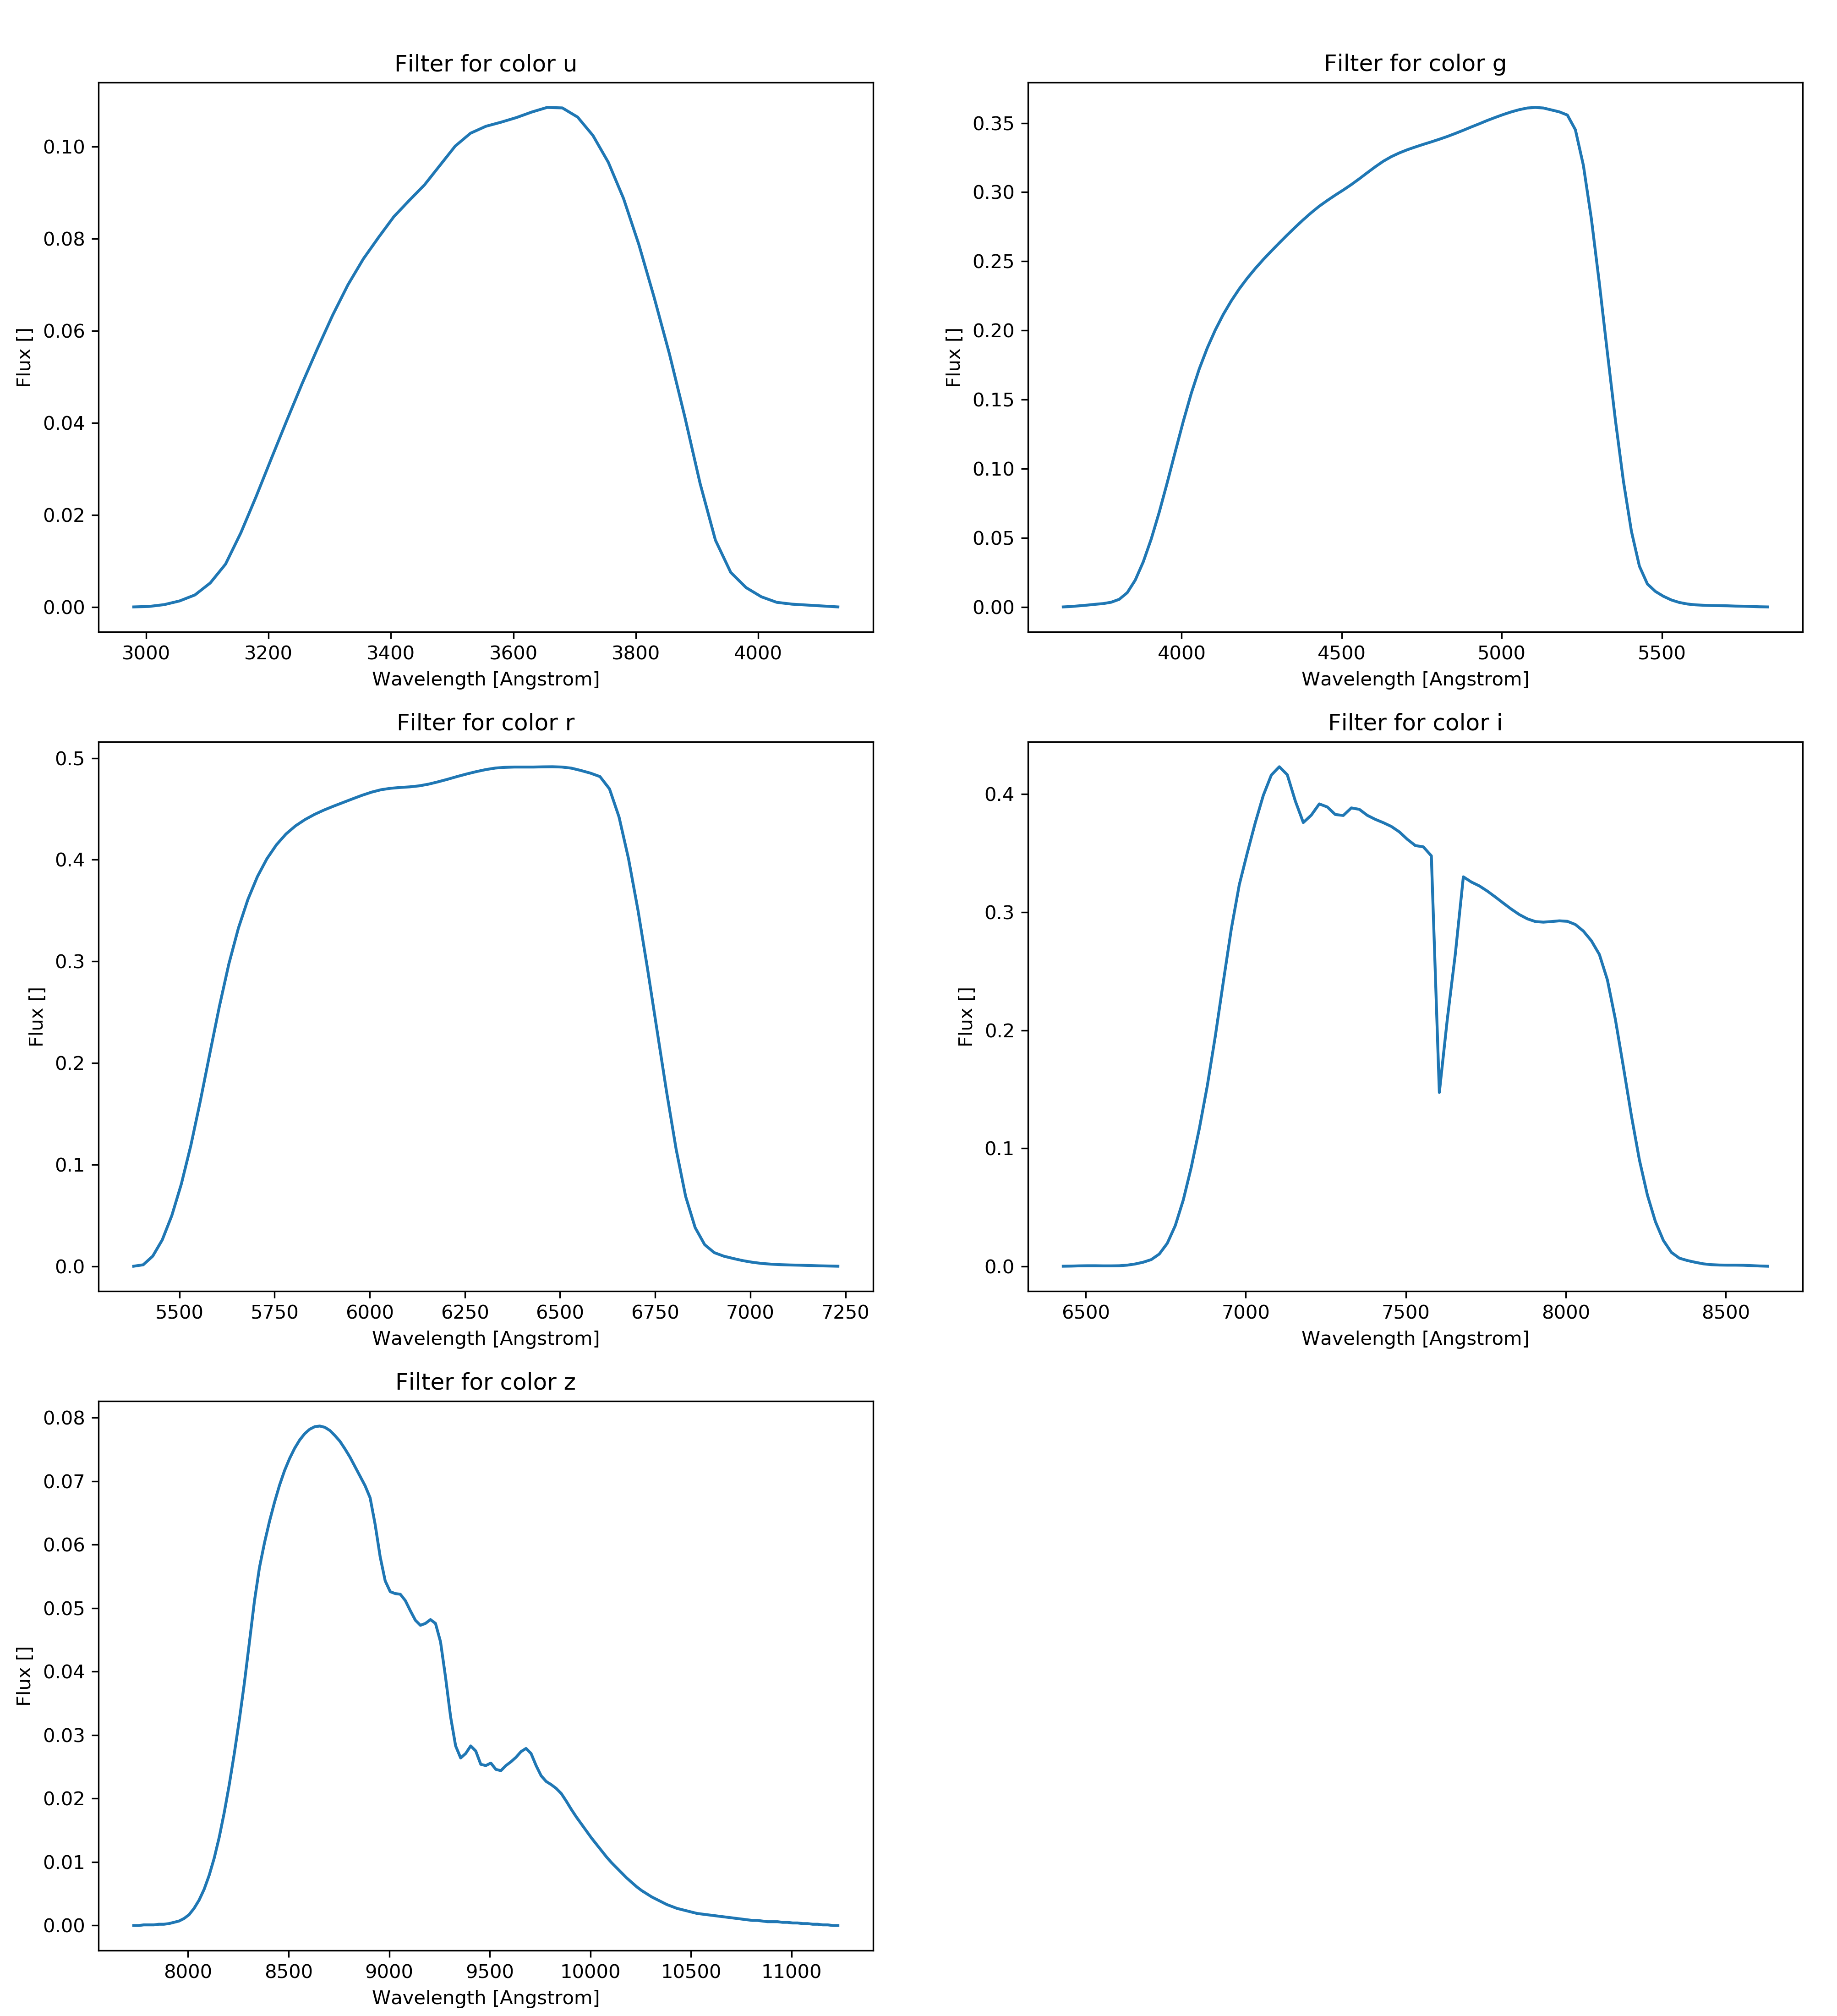
\includegraphics[width=.66\textwidth]{./filters.png}
	\caption{ Petrosian magnitudes for color space diagrams corrected for extinction }
\end{figure}

\par The AB magnitudes were calculated as:

\begin{equation}
	m_{AB} = -2.5\cdot log_{10}(F) - 48.60
\end{equation}

\par For the integrals I used the following numerical method.
I didn't re-sample the data because I couldn't find a general enough
algorithm to do that so I wrote one. Firstly I looked for the 
minimum and maximum index of the nearest wavelength in the filters 
and in the spectral distribution. When that was found, I ran through
that part of the spectral function and always multiplied the 
appropriate spectral value with the nearest filter-function value
according to the wavelength. With this method I approximated the 
integrals and took into account that the wavelengths are in $\angstrom$.

\lstset{language=Python}
\lstset{frame=lines}
\lstset{caption={Spectrum acquiery}}
\lstset{basicstyle=\scriptsize}
\begin{lstlisting}
from sklearn.neighbors import NearestNeighbors

def get_spectrum(spectrum, color_filter):
	# min/max wavelength
	min_lambda = color_filter[:,0][0]
	max_lambda = color_filter[:,0][-1]
		
	# find nearest min/max indices
	min_nearest_ind = np.abs(spectrum[:,0]-min_lambda).argmin()
	max_nearest_ind = np.abs(spectrum[:,0]-max_lambda).argmin()
		
	# integral of response function
	c = 3*10**8
	bin_width = color_filter[:,0][1] - color_filter[:,0][0]
	filter_integral = c*np.sum(color_filter[:,1]/color_filter[:,0])
	# dimension correction
	filter_integral *= 10**10
		
	flux = 0.
		
	# NN algorithm
	neigh = NearestNeighbors(n_neighbors=1, algorithm='kd_tree')
	neigh.fit(color_filter[:,0].reshape(-1, 1))
		
	for ind, val in enumerate(spectrum[:,0][min_nearest_ind:max_nearest_ind]):
		nearest_ind = neigh.kneighbors(np.array([val]).reshape(1, -1),
			 return_distance=False)[0,:][0]
		delta_flux = color_filter[:, 1][nearest_ind]*spectrum[:,1][ind]*val
		# dimension correction
		delta_flux *= 10**(-10)
		flux += delta_flux
	return -2.5*np.log10(flux/filter_integral) - 48.60
\end{lstlisting}

\par The templates were acquired from the Le Phare \cite{lephare} 
dataset and most of the galaxy templates were used. I also acquired
galaxy templates from Laszlo Dobos but I didn't use them since they 
didn't cover the whole wavelength spectrum, therefore it wouldn't have 
been possible to return all color indices as the final goal of this 
process is to deduct the appropriate color indices with the matching
redshift values.

\begin{figure}[H]
	\centering
	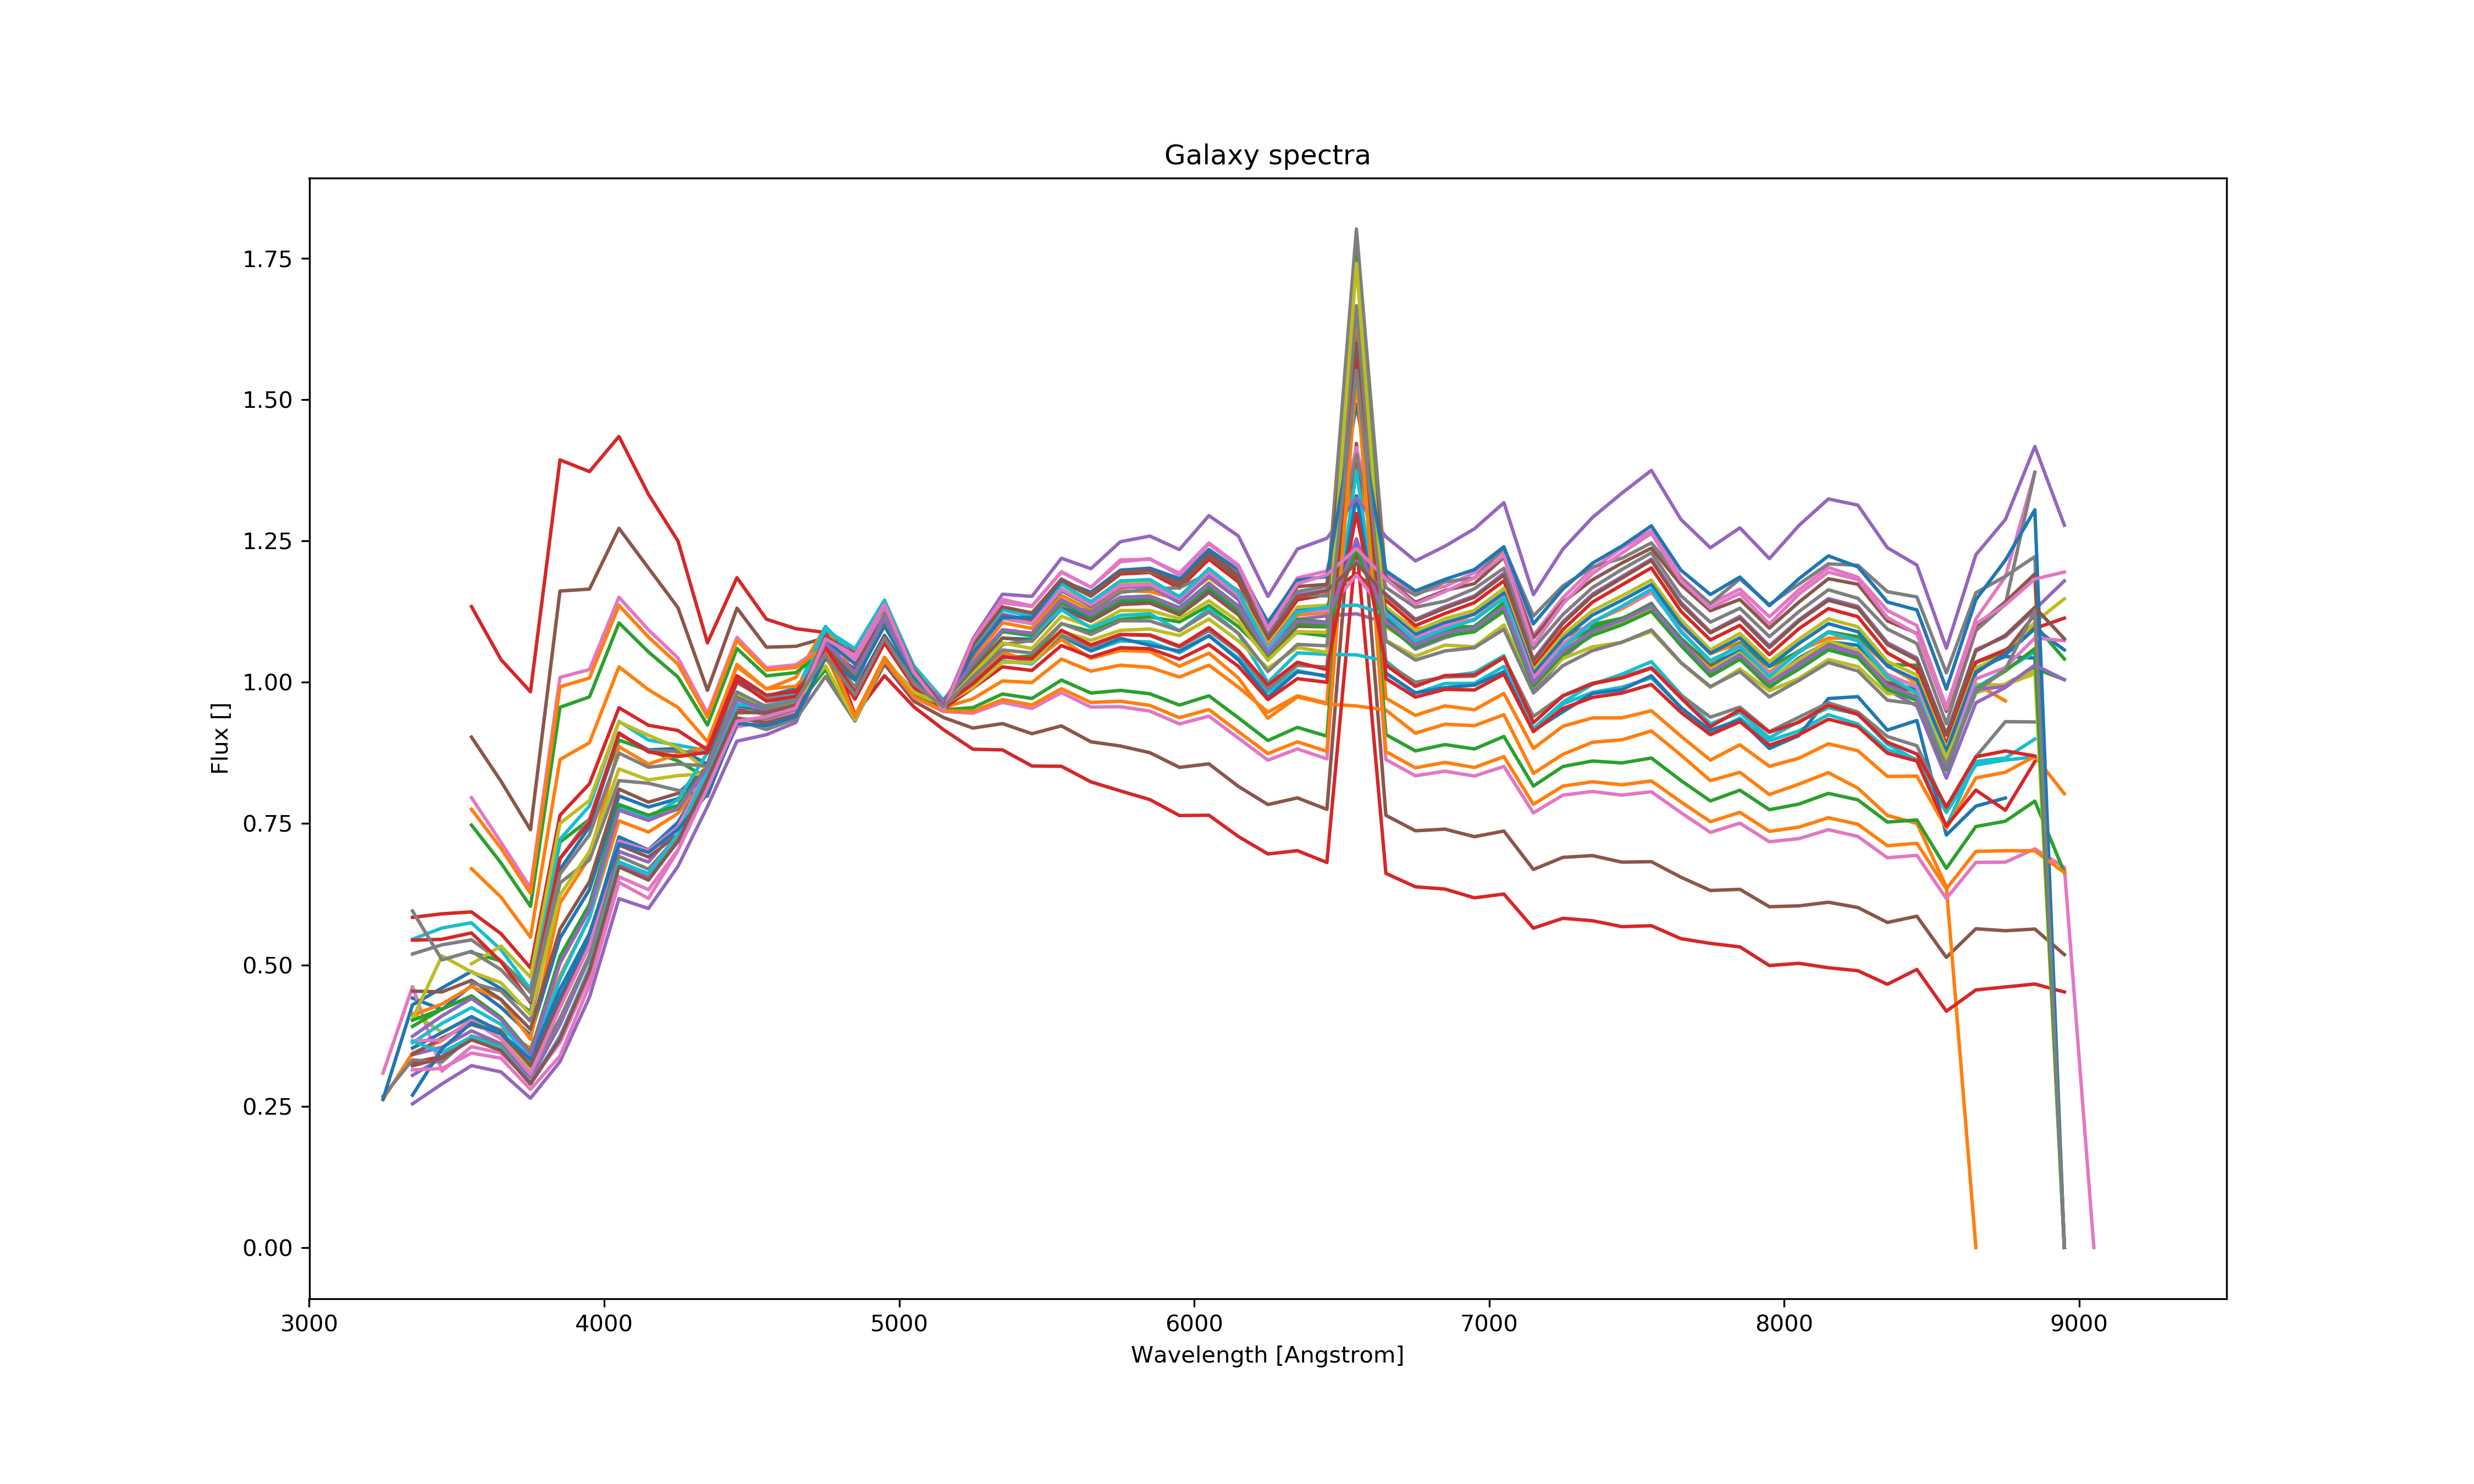
\includegraphics[width=.8\textwidth]{./dobos-spectra.png}
	\caption{ Dobos spectra from voservices }
\end{figure}

\par Using N dataset from Le Phare (N=299), applying the band filters (5)
for each of them and setting a step size (step size = 150) for incrementing
the redshift value the wavelengths were multiplied in each step and the color 
bands recalculated. This results in N*bands*step\_size data points and thus much
more calculations. This process was painfully slow therefore I was only able 
to generate at most 45 000 lines of template data and match less then half of it
using $\approx$ 800 000 lines of measured data.

\par The matching was done with KNN algorithm for the whole dataset line by 
line using \textit{sklearn} therefore it was easy and fast to match even
hugh amounts of data. Only a small portion of it ($\approx$ 20\%) was selected for further process
since most of the template data is junk and only some of it can be used as 
representative. The matching was done using the $ug, gr, ri, iz$ color indices and
the $redshift$ value. However, as it can be seen below the matched data is not correct
since it does not cover the whole color space. It is sometimes completely off, thus
those data points are excluded since they only issue > 0.5\% of the dataset.

\begin{figure}[H]
	\centering
	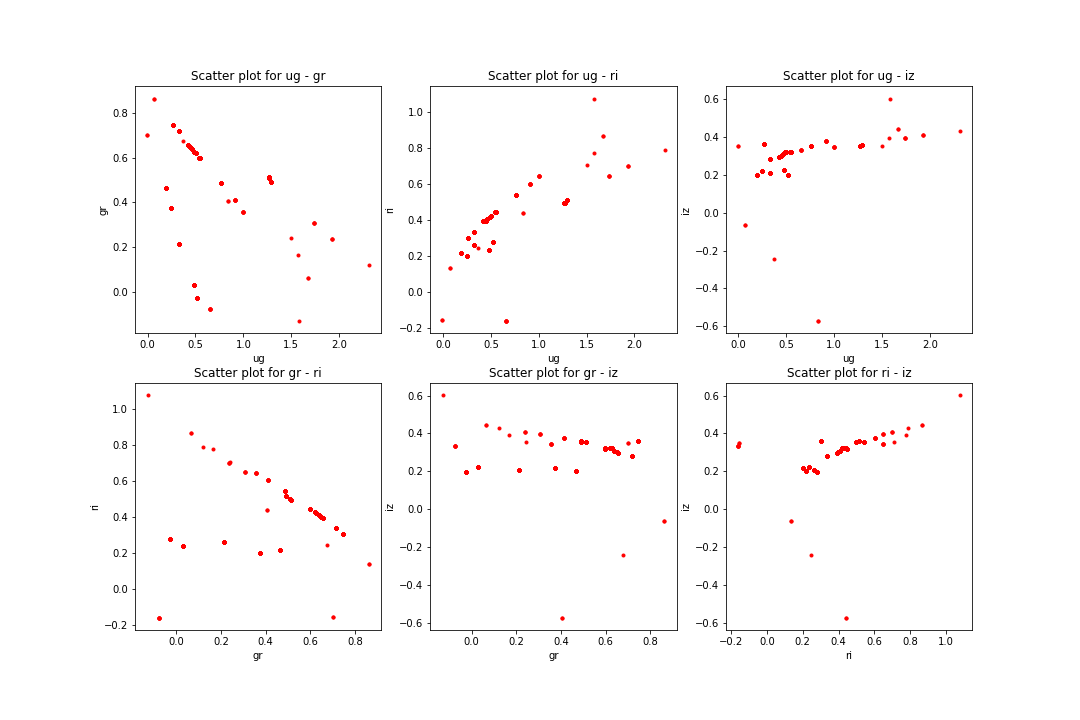
\includegraphics[width=.86\textwidth]{./colorspace.png}
	\caption{ Color space distribution of matched template data }
\end{figure}

\par It can be clearly seen that this is not the same as before 
for the measured data set and is not even close. It shows some 
resemblance to the petrosian data points but is objectively bad.
Using a 20\%-80\% train-test split and excluding the completely off
predictions the results are:

\begin{figure}[H]
	\centering
	\begin{minipage}{0.5\textwidth}
		\centering
		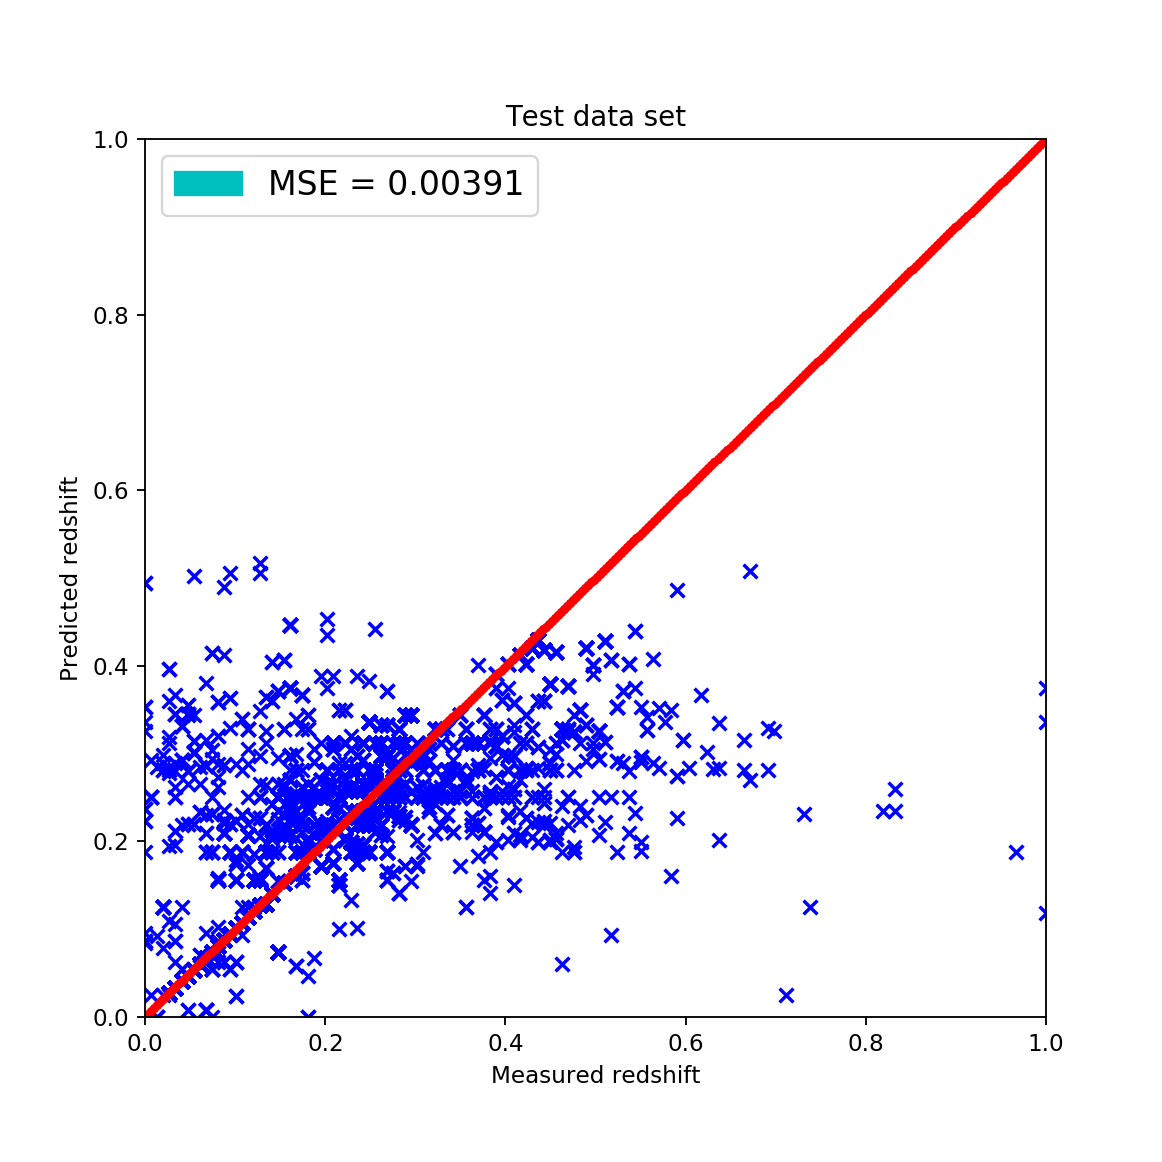
\includegraphics[width=0.95\textwidth]{./dataframe.png}
		\caption{ Result on test set }
	\end{minipage}\hfill
	\begin{minipage}{0.5\textwidth}
		\centering
		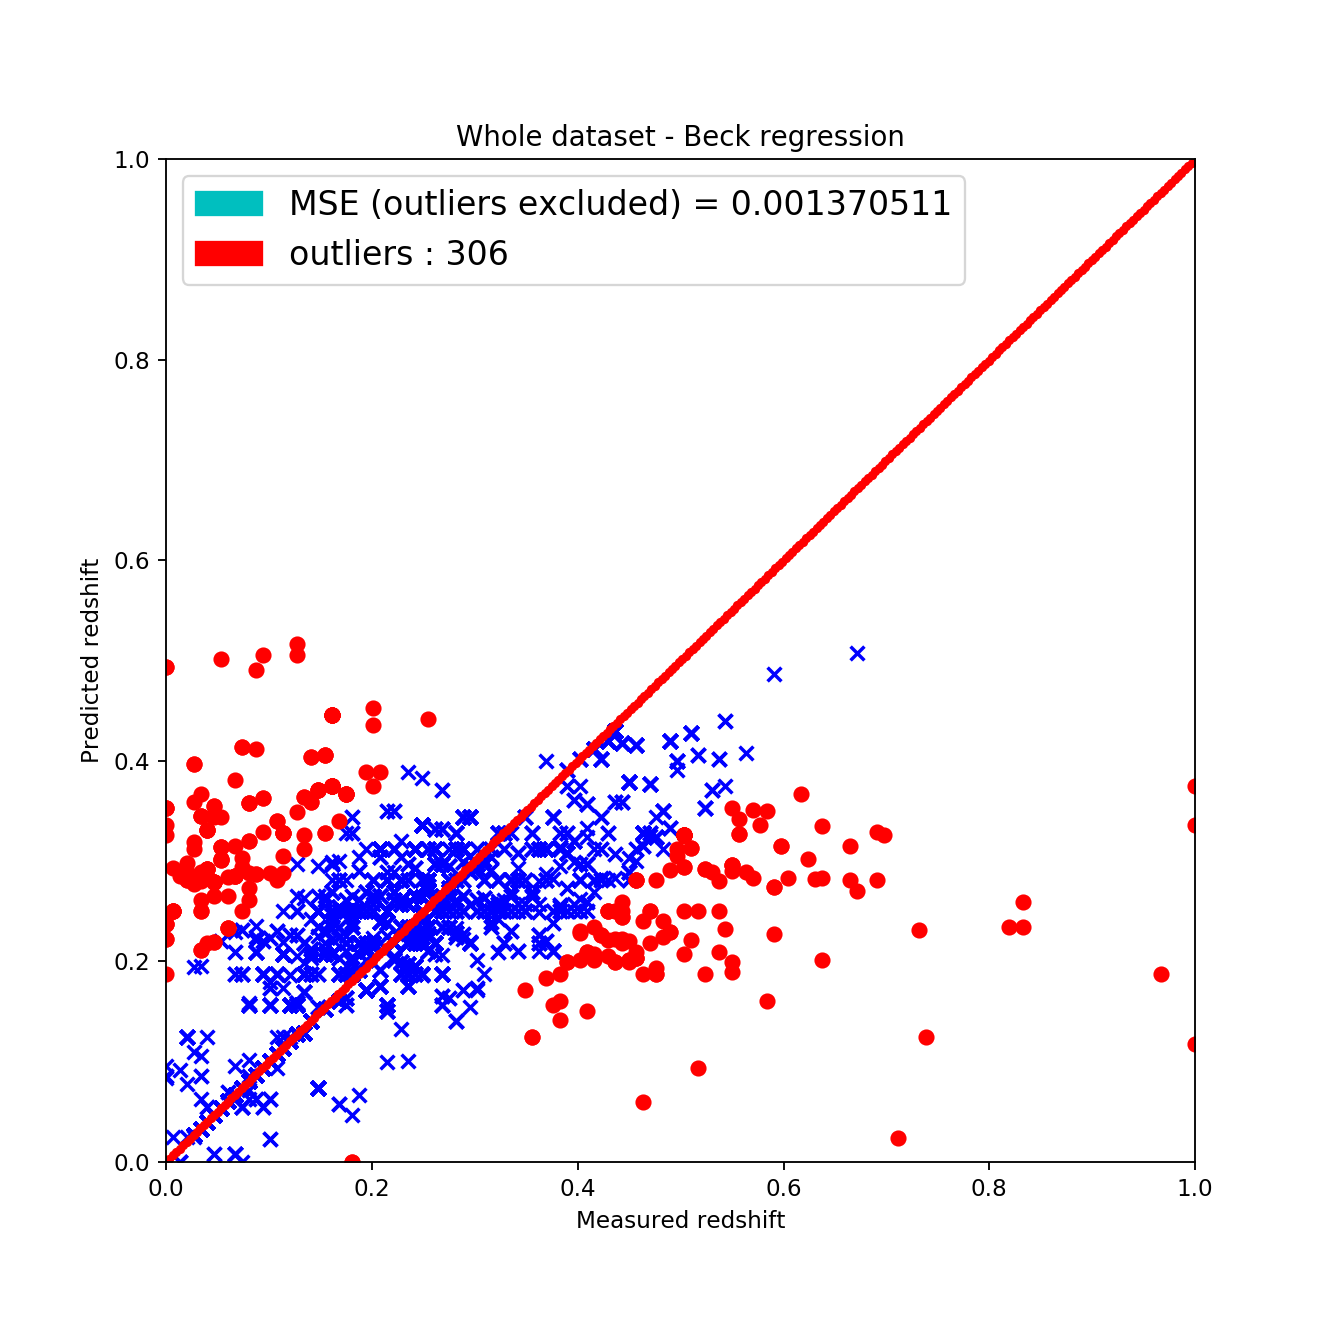
\includegraphics[width=0.95\textwidth]{./dataframe-without-outliers.png}
		\caption{ Result on dataset }
	\end{minipage}
\end{figure}

\par The matched set contained 12 000 points and around 9600 was used
as test set. Approximately 3\% of it contains outliers and > 0.5\% is completely
of by the predictor. The Beck method fails on the template set due to the 
fact that some points are amongst the points more than once and the 
linear regression can't be done properly. Also a huge issue, that 
the data points do not cover the color space at all.

\section{Overview}

\par Therefore I completed all the tasks required to finish this project. I thinks that I made 
great progress throughout the weeks and I have overdone what I had to do. However, I am sure that 
there is some kind of problem with my template fitting as it has to be bad, but not this bad. My predictions
are way off. All in all, I consider this work successful and I am happy that I could work on this. It 
raised my interest more to progress in the machine learning field further.

\par My work can be found on GitHub \cite{qbeer} and on my webapge \cite{myblog}.

\newpage
\bibliographystyle{plain}
\bibliography{references}

\end{document}